%	\item Beregninger og dimensionering af 6. ordens chebycheb filtre
%	\item Implementeringsvalg og design af hardware/schematics
%\note{Generel intro til audio signaler}

\section{Analoge filtres rolle ved digital signalbehandling}\label{sec:filter_intro}
For at kunne udføre digital signalbehandling af et analogt signal, bliver signalet overført fra den analoge verden til den digitale og tilbage igen - dette sker ved sampling og rekonstruktion.
Denne signalbehandling følger nogle faste deltrin, som kan ses i et generelt signal-blok diagram i figur \ref{fig:dsp_model}. 
\begin{figure}[h!]
	\centering
	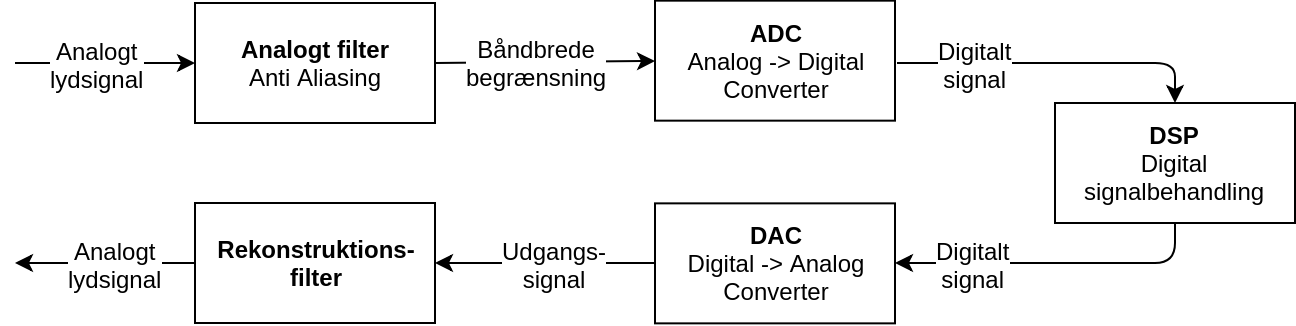
\includegraphics[width=1\textwidth]{billeder/dsp_model.png}
	\caption{DSP model.}
	\label{fig:dsp_model}
\end{figure}

Helt overordnet kan ideel sampling af et vilkårligt signal beskrives som 
\begin{align}
x_s(t) = x(t)p(t)
\end{align}
hvor $x_s(t)$ er det samplede signal, $x(t)$ er det analoge indgangssignal og $p(t)$ er en funktion af enhedsimpulser med en periode på $T_s$ (se figur \ref{fig:sampling_signal}).
\begin{figure}[h!]
	\centering
	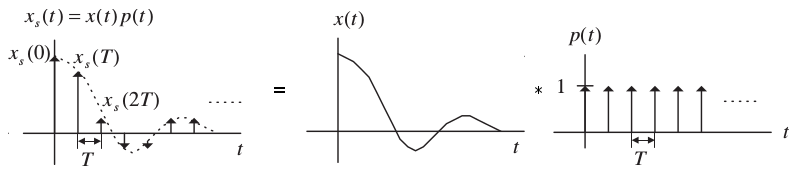
\includegraphics[width=.9\textwidth]{billeder/sampling.png}
	\caption{Ideel samplings model af signal $x(t)$. Kilde:\protect\cite[Figure 2.5 s.18 ]{Tan2013}}
	\label{fig:sampling_signal}
\end{figure}
Med udgangspunkt i en Fourier transform af det kontinuerlige og vilkårlige signal $x(t)$ 
\begin{align}
X(f) = \int_{-\infty}^{\infty}x(t)e^{-j2\pi f t}dt
\end{align}
som kan ses i figur \ref{fig:alias}(a) hvor den maksimale samplede frekvens er angivet som $B=f_{max}$.
Dette udtryk omskrives til diskret tid, ved at antage $t\curvearrowright nT_s$, hvor $n$ angiver tidsindeks i funktionen $p(t)$.
\footnote{Det antages at $T_s = 1/f_s$ er kendt og derved undlades og kun angives efterfølgende af $n$.}
\begin{align}
	X(f) = \sum_{n=-\infty}^{\infty}x(n)e^{-j2\pi f n}
\end{align}
Med en skaleret frekvensakse $\Omega = 2\pi f T_s$ kan en periodisk egenskab vises som
\begin{align}
	X(\Omega + 2\pi) = \sum_{n=-\infty}^{\infty}x(n)e^{-j(\Omega + 2\pi) n} = \sum_{n=-\infty}^{\infty}x(n)e^{-j\Omega n}
\end{align}

Således vil det diskrete frekvensspektrum gentages hvert $1/T_S$ eller $f_s$ som angiver samplefrekvensen.
I figur \ref{fig:alias}(b) vises gentagelserne i frekvensspektrummet også kaldet aliases.

\begin{figure}[h!]
	\centering
	\begin{subfigure}[b]{.7\textwidth}
		\centering
		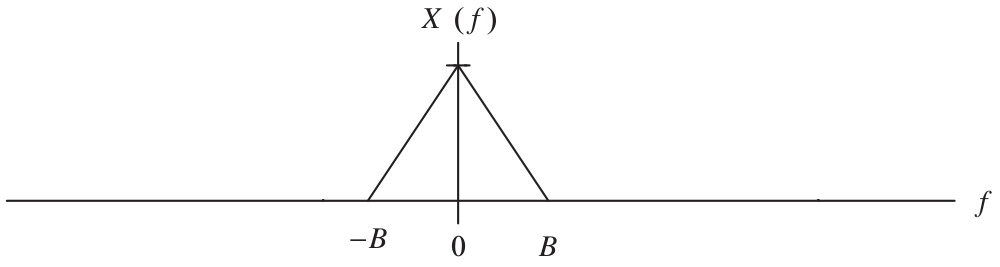
\includegraphics[width=\textwidth]{billeder/aliasing1.png}
		\label{fig:alias1}
		\caption{Fourier transform $X(f)$ af signal $x(t)$}
	\end{subfigure}
	\begin{subfigure}[b]{.7\textwidth}
		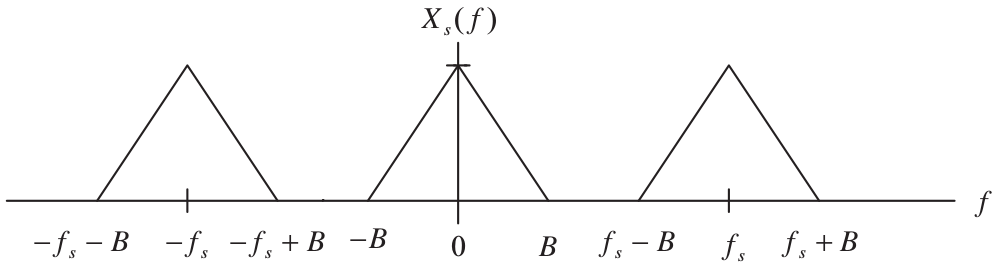
\includegraphics[width=\textwidth]{billeder/aliasing2.png}
		\label{fig:alias2}
		\caption{Diskret tids Fourier transform $X_s(f)$ af signal $x(t)$}
	\end{subfigure}
%	\begin{subfigure}[b]{.45\textwidth}
%		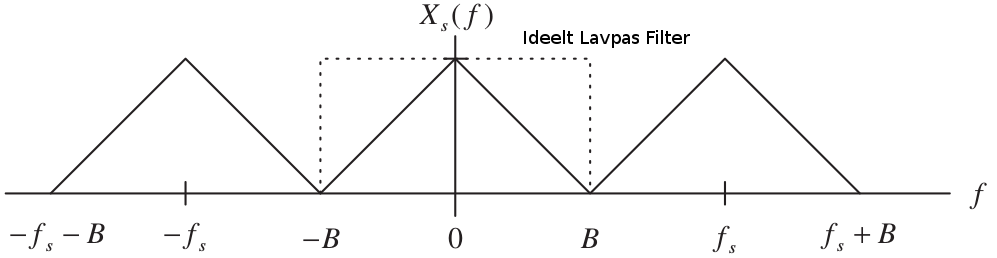
\includegraphics[width=\textwidth]{billeder/aliasing3.png}
%		\label{fig:alias3}
%		\caption{xx}
%	\end{subfigure}
	\begin{subfigure}[b]{.7\textwidth}
		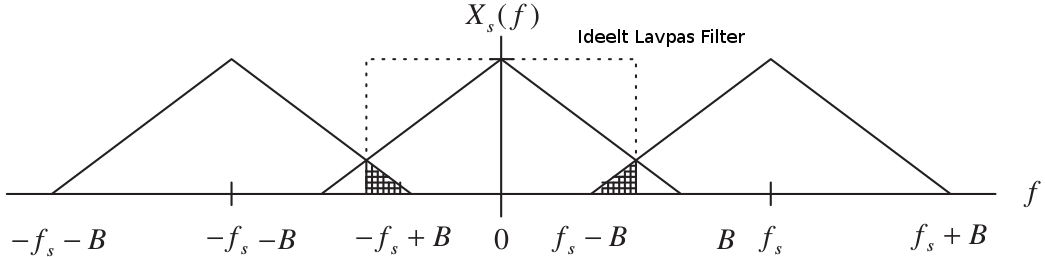
\includegraphics[width=\textwidth]{billeder/aliasing4.png}
		\label{fig:alias4}
		\caption{Diskret tids Fourier transform $X_s(f)$ med uønsket aliasing}
	\end{subfigure}
	\caption{Plot af vilkårligt signal. $B$ angiver maksimal frekvens $f_{max}$. Kilde:\protect\cite{Tan2013}}
	\label{fig:alias}
\end{figure}

Således kan det ses, at den maksimale frekvens $B$ i det ønskede samplede signal ikke må overstige $f_s/2$, også kaldet for Nyquist frekvensen.
\begin{align}
	f_{max} \leq f_s/2 \label{eq:shannons}
\end{align}
Ligning \ref{eq:shannons} er Shannons sampling theorem og intervallet mellem $-f_s/2$ og $f_s/2$ er Nyquist intervallet.
Hvis den maksimale frekvens i signalet er større end $f_s/2$ og Shannons samplings theorem derved ikke er overholdt, opstår der aliasing i det samplede signal der ses som det skraverede område i figur \ref{fig:alias}(c).
\\
I figur \ref{fig:dsp_model} fremstår det analoge filter på indgangen som en båndbredde begrænsning.
Denne begrænsning er således en nødvendighed for at undgå aliasing. 
\\
Som udgangspunkt blev opløsningen af den Analog-til-Digital Converter (ADC) brugt til at vurdere hvor meget dæmpning et analogt filter skulle have for at kunne sikre en komplet og tabsfri gengivelse af signalet.

Ud fra de fremsatte krav til projektet, benyttes der en \emph{ARM Cortex-M4F} baseret microcontroller fra Texas Instruments \cite{spmu296} der er udstyret med en 12bit ADC på de analoge indgange.
For at bestemme opløsning på ADC'en, kan den unipolære\footnote{Unipolær kvantificering skyldes ADC'ens spændingsområde på $0 \longmapsto \num{3.3}\si{\volt}$.} kvantificering $\Delta_{ADC}$ bestemmes samt Signal to Noise Ratio $SNR_Q$.
   
\begin{align}
	\Delta_{ADC} &= \frac{V_{max}}{2^N} = \frac{\num{3.3}\si{\volt}}{2^{12}} \approx \num{80.6}\si{\milli\volt}\\
	SNR_{Q,dB} &= 10 \log \left[6,02 N + 2 \right] = 10 \log \left[6,02\cdot 12+2\right] = 74,24 \si{\decibel} 
\end{align}
 
Således er det mindste målbare signal $SNR_Q$ og deraf kan konkluderes at aliasing effekten skal dæmpes med tilsvarende $74\si{\decibel}$ for at den ikke har indflydelse på det samplede signal.

Når der er tale om et audio signal, hvor det ønskede frekvensområde der ønskes bevaret er $20\si{\hertz}$ til $18\si{\kilo\hertz}$ og en samplingsfrekvens på $f_s = 44,1\si{\kilo\hertz}$ resulterer dette i en filter orden af ekstrem størrelse.

Valget faldt således på at anvende et 6. ordens filter. Dette giver et fornuftigt antal komponenter under implementeringen og den efterfølgende kortlægning af de uønskede effekter må vise om, hvorvidt det er et fornuftigt valg.  
 

\section{Analyse af filter typer}\label{sec:filter_analyse}
%\note{Gennem gang af de filter topologier der har været i betragtning som en mulig løsning.}
For at kunne finde frem til et passende lavpasfilter som anti aliasing filter, bliver fire filter typer sammenlignet - Butterworth, Chebyshev type I og II samt Bessel (Thomson).
Hver af disse filtre har en tilhørende amplitudekarakteristik der beskrives med følgende overføringsfunktioner\cite{anfilter}.

\begin{align} 
H_{butterworth}(j\omega_n) &= \frac{1}{\sqrt{1 + \omega_n^{2n}}} \label{eq:H_butt} \\
H_{bessel} (j\omega_n) &= \frac{H}{a_0 + \omega^2 + ja_1\omega_n} \label{eq:H_bes}\\
H_{chebychevI}(j\omega_n) &= \frac{1}{\sqrt{1 + \epsilon^2 C_n^2(\omega_n)}} \label{eq:H_cheb1} \\
H_{chebychevII}(j\omega_n) &= \frac{1}{\sqrt{1 + \frac{1}{\epsilon^2 C_n^2(\omega_n)}}} \label{eq:H_cheb2} \\
C_n(\omega_n) &=  
\begin{matrix}
	\cos(n\arccos(\omega_n)) & 0 \le \omega_n \le 1 \\  \cosh(n \arccosh(\omega_n)) & 1 \le \omega_n 
\end{matrix} \label{eq:chev_cn_funk}
\end{align}

I ligning (\ref{eq:chev_cn_funk}) fremgår den indre funktion $C_n(\omega_n)$ som bruges i Chebychev I og II i ligning (\ref{eq:H_cheb1}) og (\ref{eq:H_cheb2}).

Figur \ref{fig:filter_typer} viser en samlet fremstilling af amplitude karakteristikken $H(j\omega_n)$ og gruppeløbetiden $D(\omega_n)$ for de fire filtertyper.

\begin{figure}[h!]
	\centering
	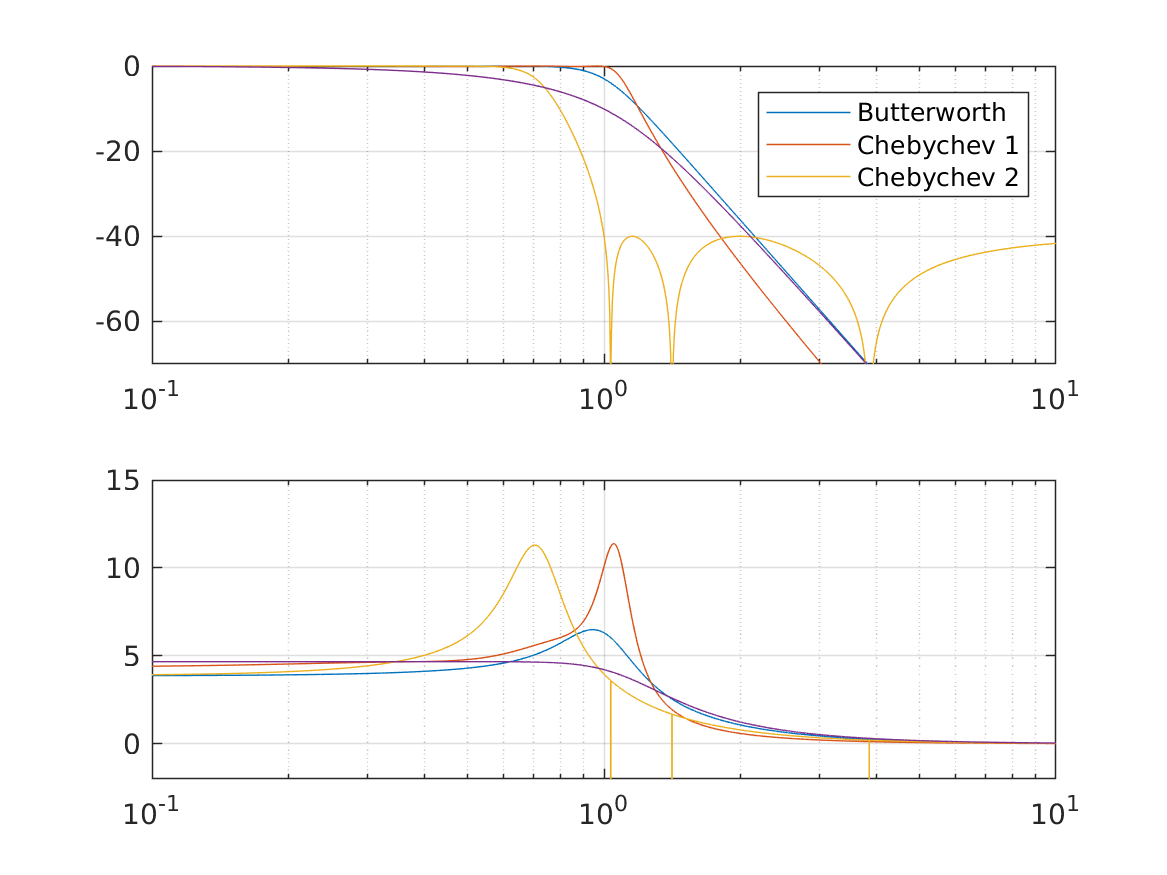
\includegraphics[width=1\textwidth]{matlab/filter_compare.png}
	\caption{Normeret 6.ordens filter karakteristik (øverst) og guppeløbetid (nederst) for filtertyperne Butterworth, Chebychev Type I ($0,1 \si{\decibel}$ ripple) \& Type II ($-40 \si{\decibel}$ stopbånds ripple) og Bessel.}
	\label{fig:filter_typer}
\end{figure}

Det ønskede filter skal have en rimelig flad karakteristik i pasbåndet og en stejl overgang til stopbåndet.
Således kan lydsignalets amplitude holdes konstant i hele det ønskede frekvensområde, da uønsket dæmpning/forstærkning af lydsignalet kan medføre hørbare ændringer af lydbilledet, på samme måde som en equalizer påvirker et lydsignal. 

Ligeledes ønskes en rimelig konstant gruppeløbetid. 
Gruppeløbetiden, der er defineret i ligning (\ref{eq:groupdelay_def})\cite{anfilter}, er et udtryk for hvor stor tidsforsinkelsen på signalet som funktion af frekvensen er.

\begin{align}
	D(\omega) \stackrel{def}{=} - \dfrac{d(arg(N(\omega)))}{d\omega}\label{eq:groupdelay_def}
\end{align}

Hvis signalforsinkelsen bliver for stor i et givet frekvensområde, vil der fremstå en hørbar ændring af lydbilledet.
Dette fænomen er dog ret subjektivt og der findes mange meninger om hvilke tærskelværdier der kan accepteres.
Ud fra en lettere gennemgang inden for området, antages en acceptabel relativ tidsforsinkelse på $D_{rel}(\omega) < -10 \si{\milli\second}$ til projektet.   

\subsection{Valg af filter topologi}
Hvis man som udgangspunkt kun fokuserer på filtrenes gruppeløbetid, ville man skulle vælge et Bessel filter. 
Bessel filteret er designet som et filter med maksimal flad fase, men har dog langt fra den ønskede dæmpning i overgangsbåndet.
Det vælges at anvende et Chebychev type I filter, der viser sig at have den bedste dæmpning i overgangsbåndet.
Det høje udsving på gruppeløbetiden for denne filtertype, som det fremgår nederst i figur \ref{fig:filter_typer}, vil på det denormaliserede filter ligger indenfor, de i projektet, acceptable værdier. 
\\
I figur \ref{fig:filter_cheb1_denorm} øverst ses den denormaliserede filterkarakteristik for det valgte filter med en pasbåndsripple på $0,1 \si{\decibel}$ og en knækfrekvens på $f_c = 18 \si{\kilo\hertz}$ og nederst ses filterets normerede gruppeløbetid. 

\begin{figure}[h!]
	\centering
	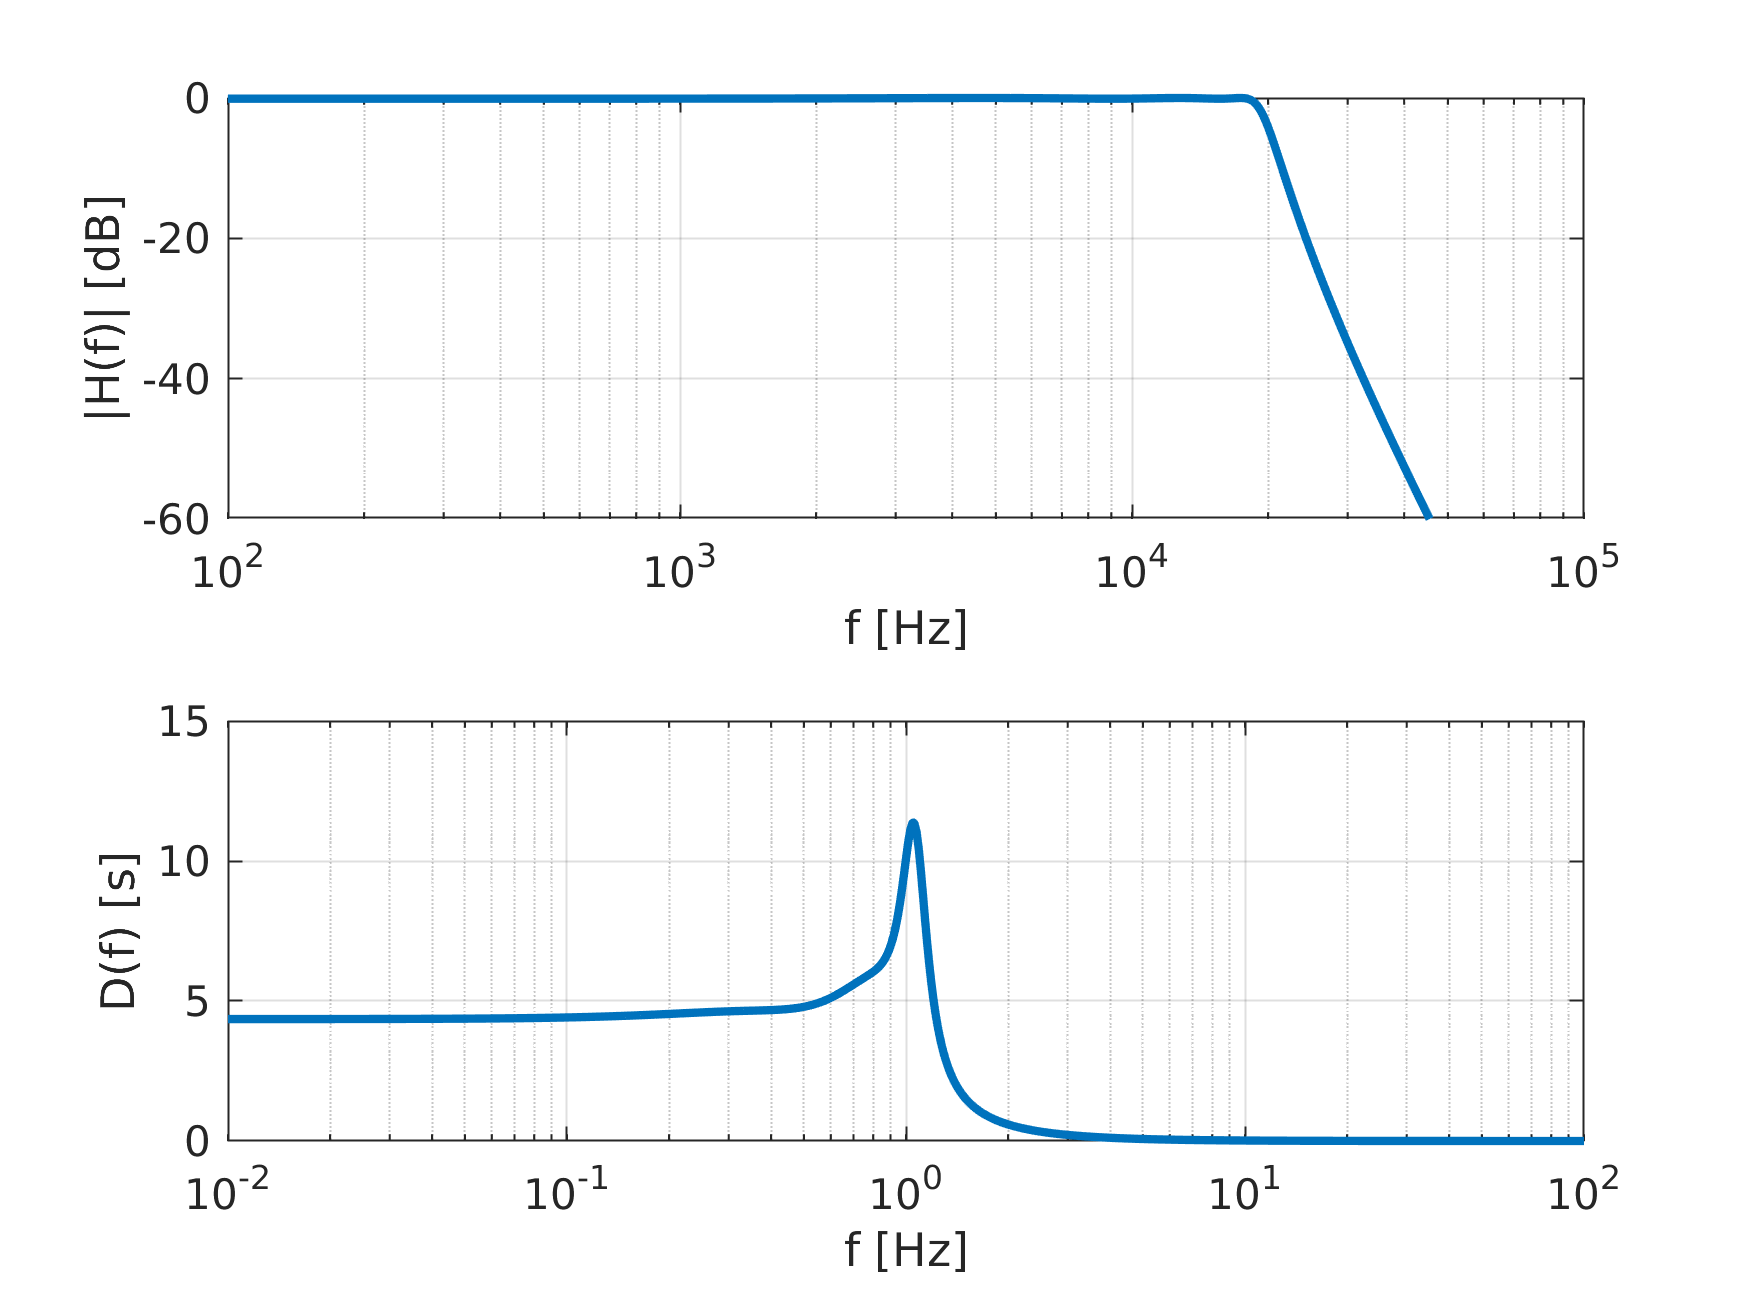
\includegraphics[width=1\textwidth]{matlab/filter_cheb1_denorm.png}
	\caption{Denormeret 6.ordens filter karakteristik og normineret guppeløbstid af Chebyshev Type I ($0,1 \si{\decibel}$}
	\label{fig:filter_cheb1_denorm}
\end{figure}

For at kunne bestemme dæmpningen af de demormaliserede filter, findes udtrykket for $|H(f)|$.
Med udgangspunkt i ligning \ref{eq:H_cheb1}, bestemmes $\epsilon$, som er bestemt ud fra ripplefaktoren i et Chebyshev filter\footnote{Figur 1.11.1 og ligning 1.11.3 i kilde \cite{anfilter}}
\begin{align}
	K_p = 20 \log \frac{1}{\sqrt{1+\epsilon^2}} \Leftrightarrow \epsilon = \sqrt{10^{K_p/10}-1}
\end{align}
Med en maksimal ripple på $K_p = 0,1 \si{\decibel}$ fås en $\epsilon$ på 
\begin{align}
	\epsilon = \sqrt{10^{0,1/10}-1} = \num{0.1526}
\end{align}

Da det ønskes at beregne $|H(f)|$ i området $f > f_c$ anvendes $C_n$ fra ligning \ref{eq:chev_cn_funk} hvor $w_n > 1$
Dæmpningen ved Nyquistfrekvensen på $f_s/2 = \num{22.05}\si{\kilo\hertz}$ kan nu bestemmes som

\begin{align}
|H(f)|_{\si{\decibel}} &= 20 \log \frac{1}{\sqrt{1+ \epsilon^2  \left[\cosh(n \arccosh k )\right]^2 }} \quad, \quad k = \frac{f}{f_c} \\
|H(22,05\si{\kilo\hertz})|_{\si{\decibel}} &= 20 \log \frac{1}{\sqrt{1+ 0,1526^2  \left[\cosh(n \arccosh \frac{22,05\si{\kilo\hertz}}{18\si{\kilo\hertz}} )\right]^2 }} = \num{-12.2568} \si{\decibel}
\end{align}

\subsection{Forventet aliasing ved valgte filter type}
I figur \ref{fig:filter_f_fs} ses amplitude karakteristikken $|H(f)|$ af det valgte filter med blåt og den første periodiske gentagelse af frekvens spektrum $|H(f-f_s)|$ med rødt.
\begin{figure}[h!]
	\centering
	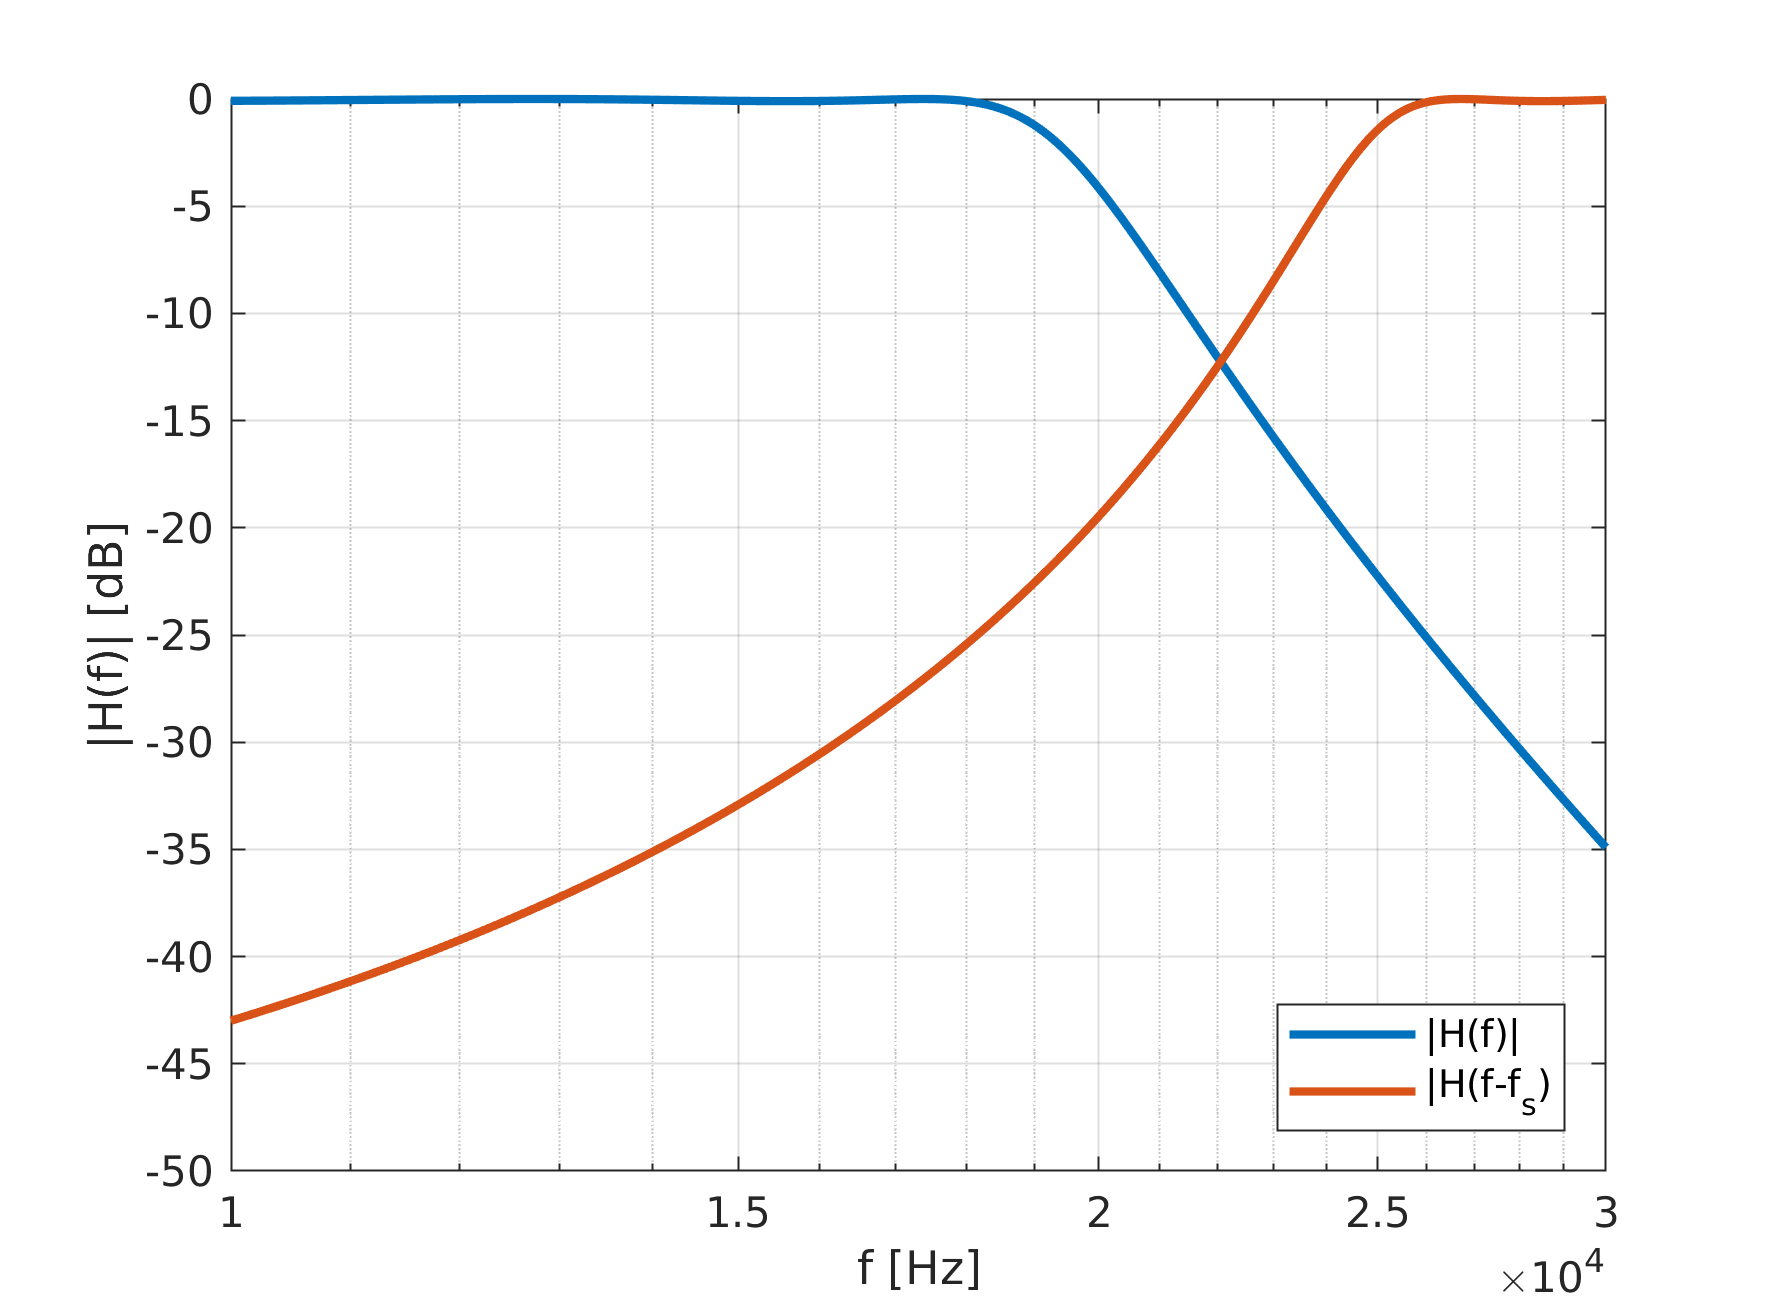
\includegraphics[width=.8\textwidth]{matlab/filter_f_fs.png}
	\caption{}
	\label{fig:filter_f_fs}
\end{figure}

En dæmpning på kun $\num{12.3} \si{\decibel}$ ved Nyquistfrekvensen er ikke ret stor og der må derfor ventes aliasing i signalet.
Størrelsen af aliasing i signalet $SA$, kan beregnes som procentvis del ved
\begin{align}
	\%SA = \frac{|H(f)|_{f=f_s-f_x}}{|H(f)|_{f=f_x}} \cdot 100 \% \label{eq:signal_alias}
\end{align} 
I ligning \ref{eq:signal_alias} angiver $f_x$ den frekvens, hvor den procentvise aliasing effekt ønskes beregnet.
Effekten kan evalueres ved at plotte $SA(f)$ fra ligning \ref{eq:signal_alias} som ses i figur \ref{fig:filter_sa}, både angivet som procentvis forhold og absolut i decibel.
Her er det således muligt at se, at der ved fx $f_c=\num{18}\si{\kilo\hertz}$ er en aliasing effekt på $5,4\%$.

\begin{figure}[h!]
	\centering
	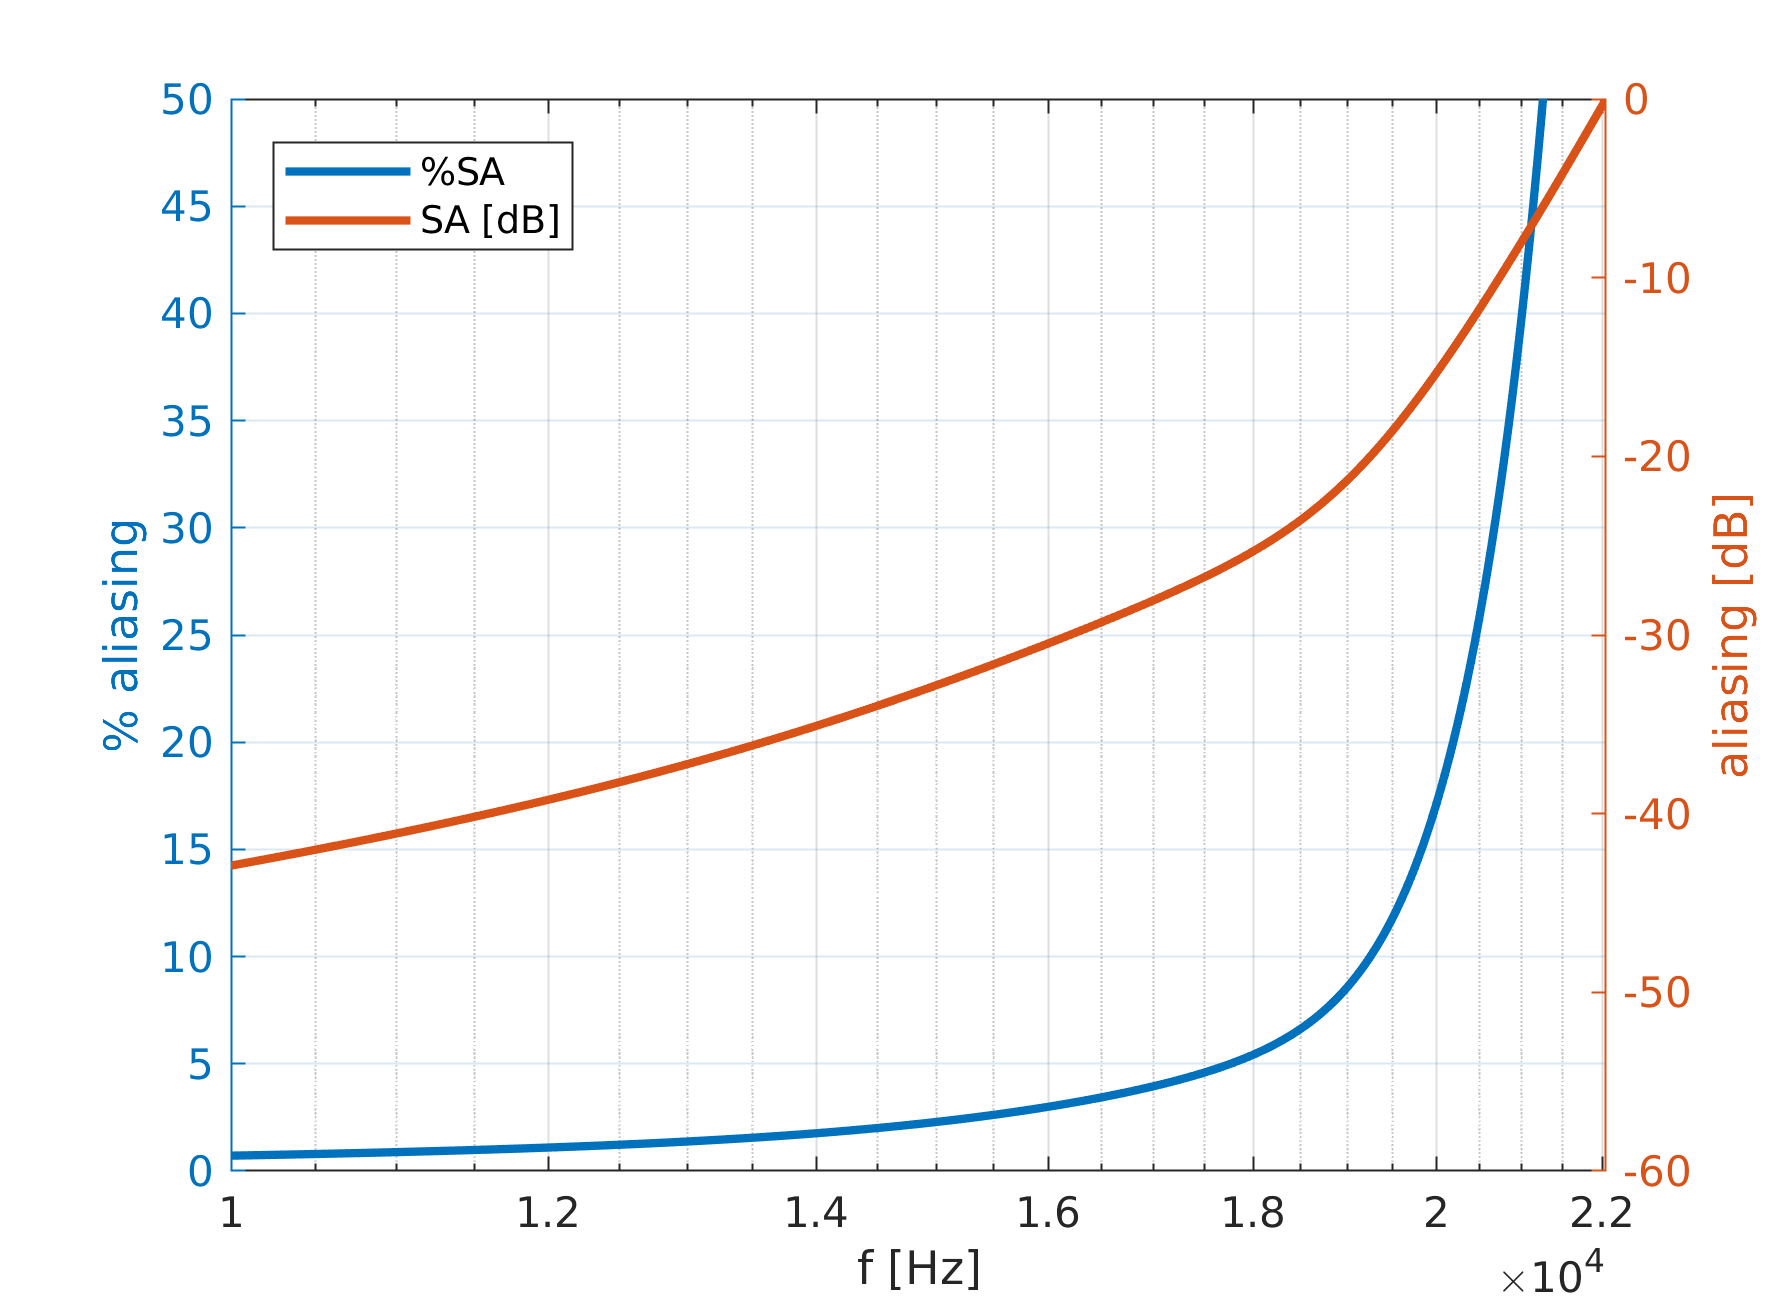
\includegraphics[width=.8\textwidth]{matlab/filter_sa.png}
	\caption{}
	\label{fig:filter_sa}
\end{figure}

%\note{Beregninger og argumentation for SNR}

\section{Specifikation og dimensionering}\label{sec:filter_spec}
Specifikationen og dimensioneringen af filteret blev udført ved hjælp af Matlab. Det samlede script kan ses i bilag \ref{bilag:aafilterspec}.

Ved at anvende Matlab funktionen \texttt{[z,p,k] = cheb1ap(n,Rp)}, fremstilles en normaliseret Chebyshev type I filter prototype. 
Parameteren \texttt{n} angiver filterets orden og \texttt{Rp} den ønskede pasbåndsripple i $\si{\decibel}$. 
Prototypen er normaliseret igennem punktet
\begin{align}
 |H(\omega)|_{\omega=\omega_0=1}=10^{-Rp/20}
\end{align}
De resulterende poler og nulpunkter oversættes derefter til en samling af 2. ordens systemer. 
En samlet overføringsfunktion kan fremstilles, men giver ingen direkte værdi udover dens anvendelighed i Matlab.
\\
De resulterende 2. ordens systemer, der ses i ligning \ref{eq:sos_h1}, \ref{eq:sos_h2} og \ref{eq:sos_h3}, kan således kaskadekobles til det samlede filter som beskrevet i ligning \ref{eq:sos_cascade}. 
\begin{align}
H_1 &= \frac{\num{0.2048}}{s^2 + \num{0.8561} s + \num{0.2634}} \label{eq:sos_h1}\\
H_2 &= \frac{\num{1}}{s^2 + \num{0.6267} s + \num{0.6964}} \label{eq:sos_h2}\\
H_3 &= \frac{\num{1}}{s^2 + \num{0.2294} s + \num{1.129}} \label{eq:sos_h3}\\
H &= H_1 \cdot H_2 \cdot H_3 \label{eq:sos_cascade}
\end{align}


Ud fra standard overføringsfunktionen for et 2. orden lavpas filter, ligning \ref{eq:stdnothlp}, kan Q-værdien og $\omega_0$ findes 

\begin{equation}
\label{eq:stdnothlp}
H_{LP}(s) = \frac{G\omega_0^2}{s^2 + \left(\frac{\omega_0}{Q}\right)s + \omega_0^2}
\end{equation}

De fundne $Q$ og $\omega_o$ værdier for det normerede filter er således
\begin{align}
	Q_1 &= \num{0.5995} \quad , \quad \omega_1= \num{0.5132} \nonumber \\
	Q_2 &= \num{1.3316} \quad , \quad \omega_2= \num{0.8345} \nonumber \\
	Q_3 &= \num{4.6329} \quad , \quad \omega_3= \num{1.0627} \label{eq:q_and_w_norm}
\end{align}

\subsection{Sallen-Key}

De analoge filtre bliver implementeret som aktive filtre. Dette er valgt da det så ikke er nødvendigt at skulle anvende spoler, da disse ofte fylder meget.
Samtidigt er de nemme at implementere da systemet i forvejen har strømforsyning til mikroprocessoren, som kan anvendes til filtrenes operationsforstærker.

Aktive filtre opbygges generelt af 2. ordens bi-quad filtre, der kaskadekobles til den ønskede orden.
I dette tilfælde seriekobles 3 filtre. 

%\note{Sallen Kay - metode 4 i afs matr.}
%\note{hvor tæt ligger de beregnede komponent værdier i hold til de anvendte tabelværdier ?}
%\note{Argumenteret valg er OpAmp -> den bedste der var som SMD}
%\note{Kort begrundelse for enkelt R i metoden og brug af op til 4 stk. C som proto type -> hvordan ville det se ud hvis kun brugte den nærmeste C i serien og hvor stor indflydelse vil det have. Måske Sensitivitesmetoden eller H(jw) -> var det er klogt valg og måske lidt overdrevet.}

Her er det valgt at anvende Sallen-Key lavpas biquads,
da disse kan realiseres ved hjælp af flere forskellige designmetoder, præsenteret 
i læreborgen 'Analog filters, second edition'\cite{KendallSu}.
En generisk Sallen-Key lavpas biquad ser ud som i figur \ref{fig:sklpbq}.

\begin{figure}[H]
	\centering
	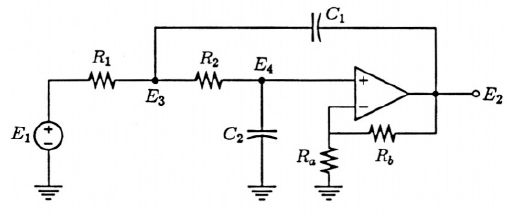
\includegraphics[width=.6\textwidth]{billeder/sklpbq}
	\caption{Sallen-Key lavpas biquad \cite{KendallSu}}
	\label{fig:sklpbq}
\end{figure}

Det blev valgt at anvende design metode 4 fra litteraturen, minimum sensitivitet.
Denne designmetode gør filteret mindre sensitivt over for variationer i komponenter ved bl.a.
at anvende enhedsforstærkning for derfor at undvære $R_a$ og $R_b$.
Det vælges at $R_1 = R_2$ der fastsættes til $1\si{\ohm}$. Herefter findes $C_1$ og $C_2$ ved hjælp af ligning \ref{eq:dm4c1} og \ref{eq:dm4c2}.

\vspace{15pt}

\begin{minipage}{0.5\linewidth}
	\begin{equation}
	\label{eq:dm4c1}
	C_1 = \frac{2Q}{\omega_0}
	\end{equation}
\end{minipage}
\begin{minipage}{0.5\linewidth}
	\begin{equation}
	\label{eq:dm4c2}
	C_2 = \frac{1}{2Q\omega_0}
	\end{equation}
\end{minipage}

\vspace{15pt}

Denne designmetode giver en stor spredning i kondensator værdierne, som er afhængig af filterets Q-værdi, som ses i ligning
\ref{eq:kondspred}.

\begin{equation}
\label{eq:kondspred}
\frac{C_1}{C_2} = 4Q^2
\end{equation}

Med de beregnede $Q$ og $\omega_o$ i ligning \ref{eq:q_and_w_norm}, kan $C_{n1}$ og $C_{n2}$ bestemmes.
Resultatet ses i tabel \ref{tab:sallen_key} kolonne 1 og 2.
\\
\\
Under arbejdet med filterdesign opstod der en fortolkningsfejl mellem den anvendte designmetode og de beregnede 2. ordens systemer fra Matlab.
Dette resulterede i en amplitude karakteristik på det valgte 6. ordens filter som ikke stemte overens med forventningerne.
Således blev et andet sæt normaliserede kondensator værdier anvendt til fremstillingen af løsningens bi-quad filter print.
De anvendte værdier ses i tabel \ref{tab:sallen_key} kolonne 3 og 4 og er taget fra \cite[Table B-2: Capacitor Values for 0.1-dB Chebyshev lowpass Sallen-Key filters, n=6]{sk_data_web}
\todo[EC]{er det meningen at denne reference skal se sådan her ud?}
\begin{table}[h!]
	\centering
	\caption{Normerede kondensator værdier for Chebyshev LPF Type I Sallen-Key, $0,1\si{\decibel}$ ripple.}
	\label{tab:sallen_key}
	\begin{threeparttable}
		\begin{tabular}{l c c c c}
			\toprule
			& \multicolumn{2}{c}{\textbf{Matlab værdier}} & \multicolumn{2}{c}{\textbf{Tabel værdier\tnote{(*)}}} \\ 
			\midrule
			\textbf{Filter \#} &
			\textbf{$C_{1n}$} 	& 
			\textbf{$C_{2n}$}  	&
			\textbf{$C_{1n}$} 		& 
			\textbf{$C_{2n}$} 	\\
			\midrule
			1 & \num{2.3362} & \num{1.6253} & \num{2.553} & \num{1.776} \\
			2 & \num{3.1913} & \num{0.4500} & \num{3.487} & \num{0.4917} \\
			3 & \num{8.7189} & \num{0.1016} & \num{9.531} & \num{0.1110} \\
			\bottomrule
		\end{tabular}
		
		\begin{tablenotes}
			\item[*] \cite[Table B-2: Chebyshev lowpass Sallen-Key filters, n=6]{sk_data_web}.
		\end{tablenotes}
	\end{threeparttable}
\end{table}

Denormering og impedans tilpasning af komponenterne gøres ud fra følgende
\begin{align}
	R &= R_n \cdot Z_n \\
	C &= \frac{C_n}{\Omega_n} \quad , \quad \Omega_n = 2\pi f_p 
\end{align} 
Det er valgt at bruge $Z_n = \num{10E3}$ og $f_p = 18\si{\kilo\hertz}$.
De endelige komponentværdier kan alle ses i det samlede diagram i bilag \ref{bilag:diagram}.